\section{KẾT QUẢ VÀ THẢO LUẬN}
\label{sec:results}
% =============================================================================

\subsection{Phân tích Dữ liệu}

Bảng~\ref{tab:descriptive} tóm tắt thống kê mô tả cho bảy biến số chính của tập dữ liệu gốc.
\texttt{Usage\_kWh} có độ lệch chuẩn lớn ($\sigma = 44{,}32$) và phân phối lệch phải mạnh (skewness $> 1$),
phản ánh sự đa dạng của các chế độ vận hành từ không tải đến quá tải cực đoan.
\texttt{CO2(tCO2)} chỉ có 8 giá trị khác biệt, xác nhận đây là biến tính toán phái sinh (emission factor $	imes$ energy),
không phải đo trực tiếp.

\begin{table}[htbp]
\caption{THỐNG KÊ MÔ TẢ DỮ LIỆU GỐC}
\label{tab:descriptive}
\centering
\small
\begin{tabular}{@{}lrrrrr@{}}
\toprule
Biến & Trung bình & Độ lệch chuẩn & Min & Max & Giá trị khác biệt \\
\midrule
\texttt{Usage\_kWh} & 27,39 & 33,44 & 0,00 & 157,18 & 3.343 \\
\texttt{Lagging\_Current\_Reactive.Power\_kVarh} & 13,04 & 16,31 & 0,00 & 96,91 & 1.954 \\
\texttt{Leading\_Current\_Reactive\_Power\_kVarh} & 3,87 & 7,42 & 0,00 & 27,76 & 768 \\
\texttt{CO2(tCO2)} & 0,012 & 0,016 & 0,000 & 0,070 & 8 \\
\texttt{Lagging\_Current\_Power\_Factor} & 0,81 & 0,19 & 0,00 & 1,00 & 5.079 \\
\texttt{Leading\_Current\_Power\_Factor} & 0,84 & 0,30 & 0,00 & 1,00 & 3.366 \\
\texttt{NSM} & 42.750 & 24.940 & 0 & 85.500 & 96 \\
\bottomrule
\end{tabular}
\end{table}

Phân tích chuỗi thời gian (Fig.~\ref{fig:timeseries}) cho thấy ba đặc điểm rõ rệt:
(i) chu kỳ ngày với đỉnh tiêu thụ tập trung trong khung giờ làm việc 8h--18h;
(ii) chu kỳ tuần với tiêu thụ ngày làm việc cao gấp khoảng 2 lần cuối tuần;
và (iii) tính mùa vụ với mùa đông có tiêu thụ cao hơn do nhu cầu sưởi ấm.
Các điểm bất thường (anomaly) được đánh dấu bằng màu sắc khác biệt,
cho thấy chúng thường xuất hiện tại các điểm chuyển tiếp chế độ vận hành hoặc khung giờ nghỉ.

\begin{figure}[htbp]
\centering
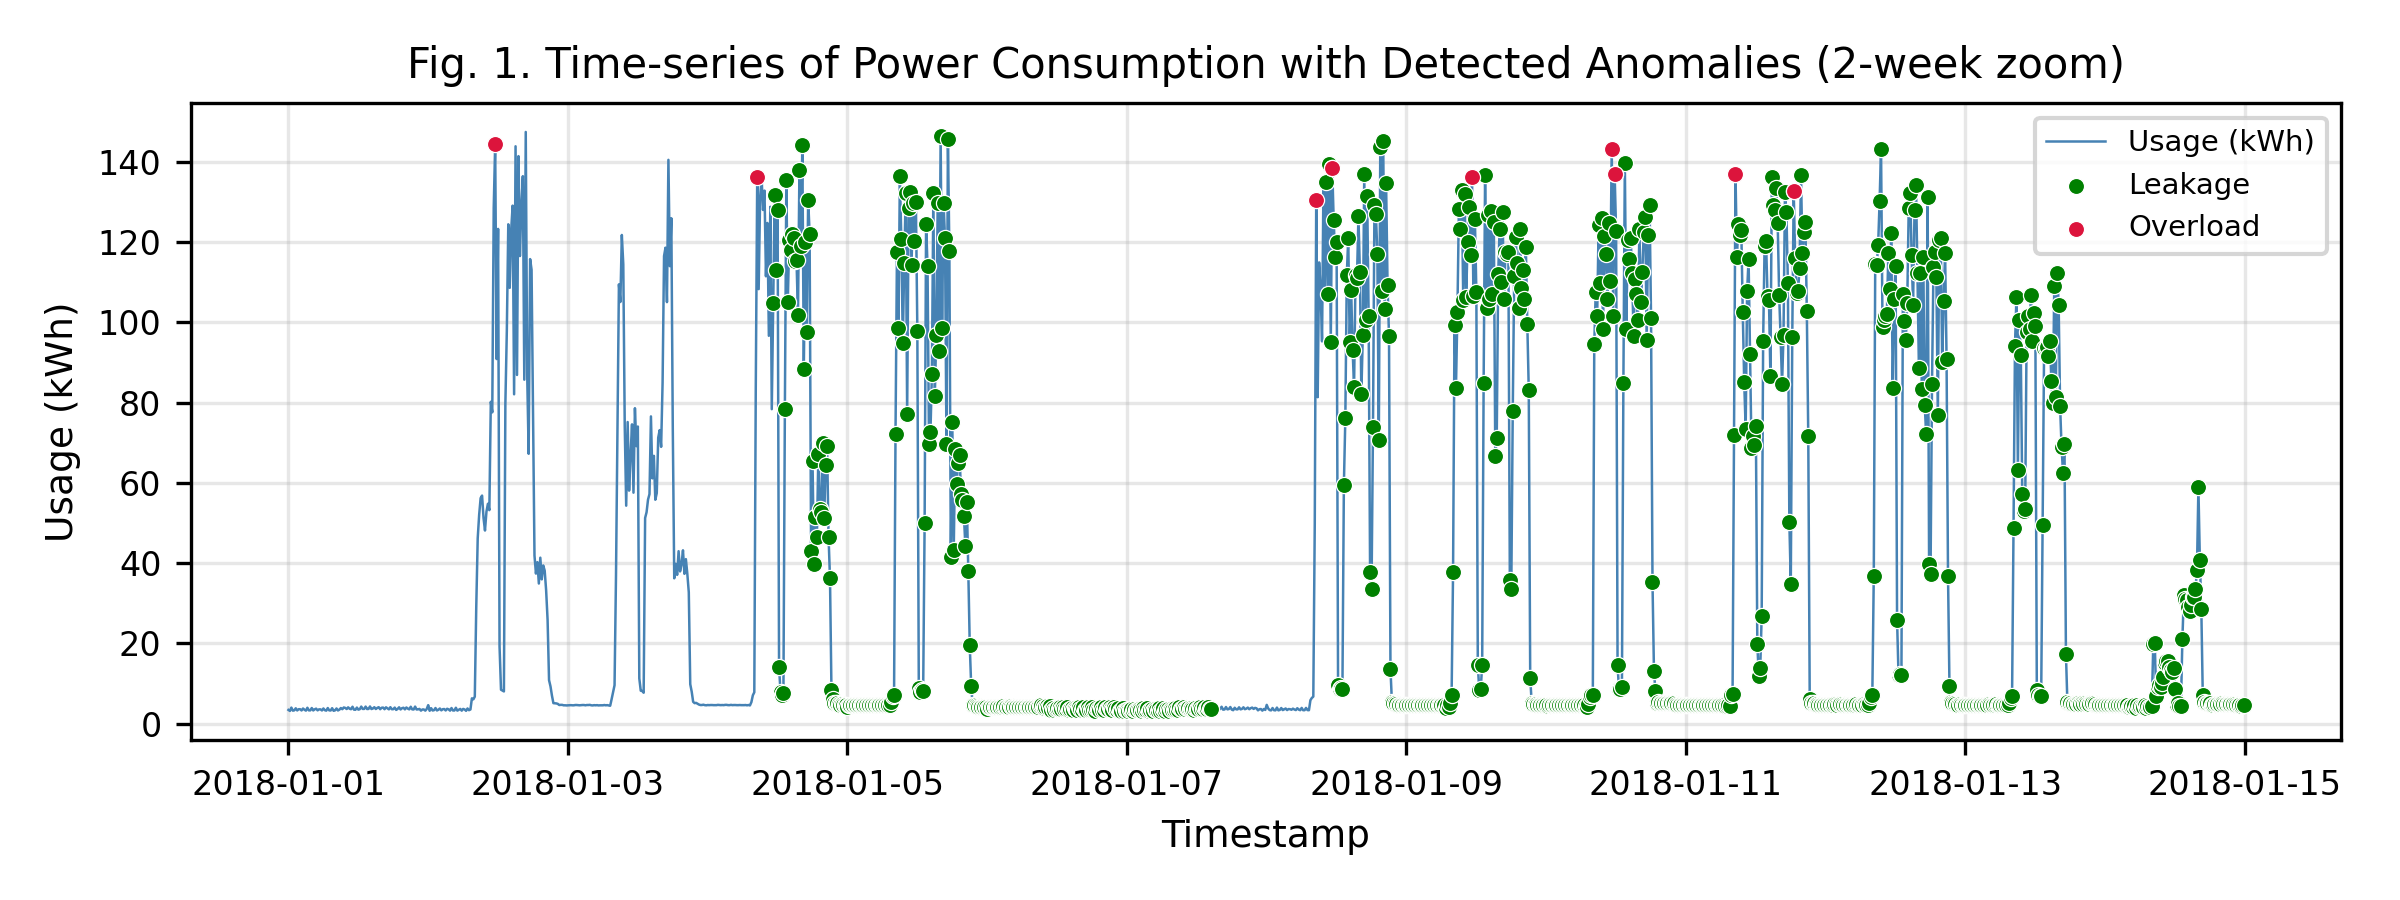
\includegraphics[width=\linewidth]{figures/fig01_time_series.png}
\caption{Chuỗi thời gian tiêu thụ điện (2 tuần đầu) với overlay ba loại bất thường.}
\label{fig:timeseries}
\end{figure}

\subsection{Đánh giá Kỹ thuật Đặc trưng}

Ma trận tương quan (Fig.~\ref{fig:heatmap}) cho thấy \texttt{Usage\_kWh} tương quan dương mạnh với \texttt{CO2} ($r \approx 0{,}95$) và \texttt{Lagging\_Current\_Reactive.Power\_kVarh} ($r \approx 0{,}78$),
phù hợp với quan hệ vật lý $S = \sqrt{P^2 + Q^2}$.
Đáng chú ý, \texttt{Leading\_Current\_Reactive\_Power\_kVarh} có tương quan yếu với các biến khác,
phản ánh đặc thù của nhà máy thép sử dụng chủ yếu tải cảm kháng (inductive load).

\begin{figure}[htbp]
\centering
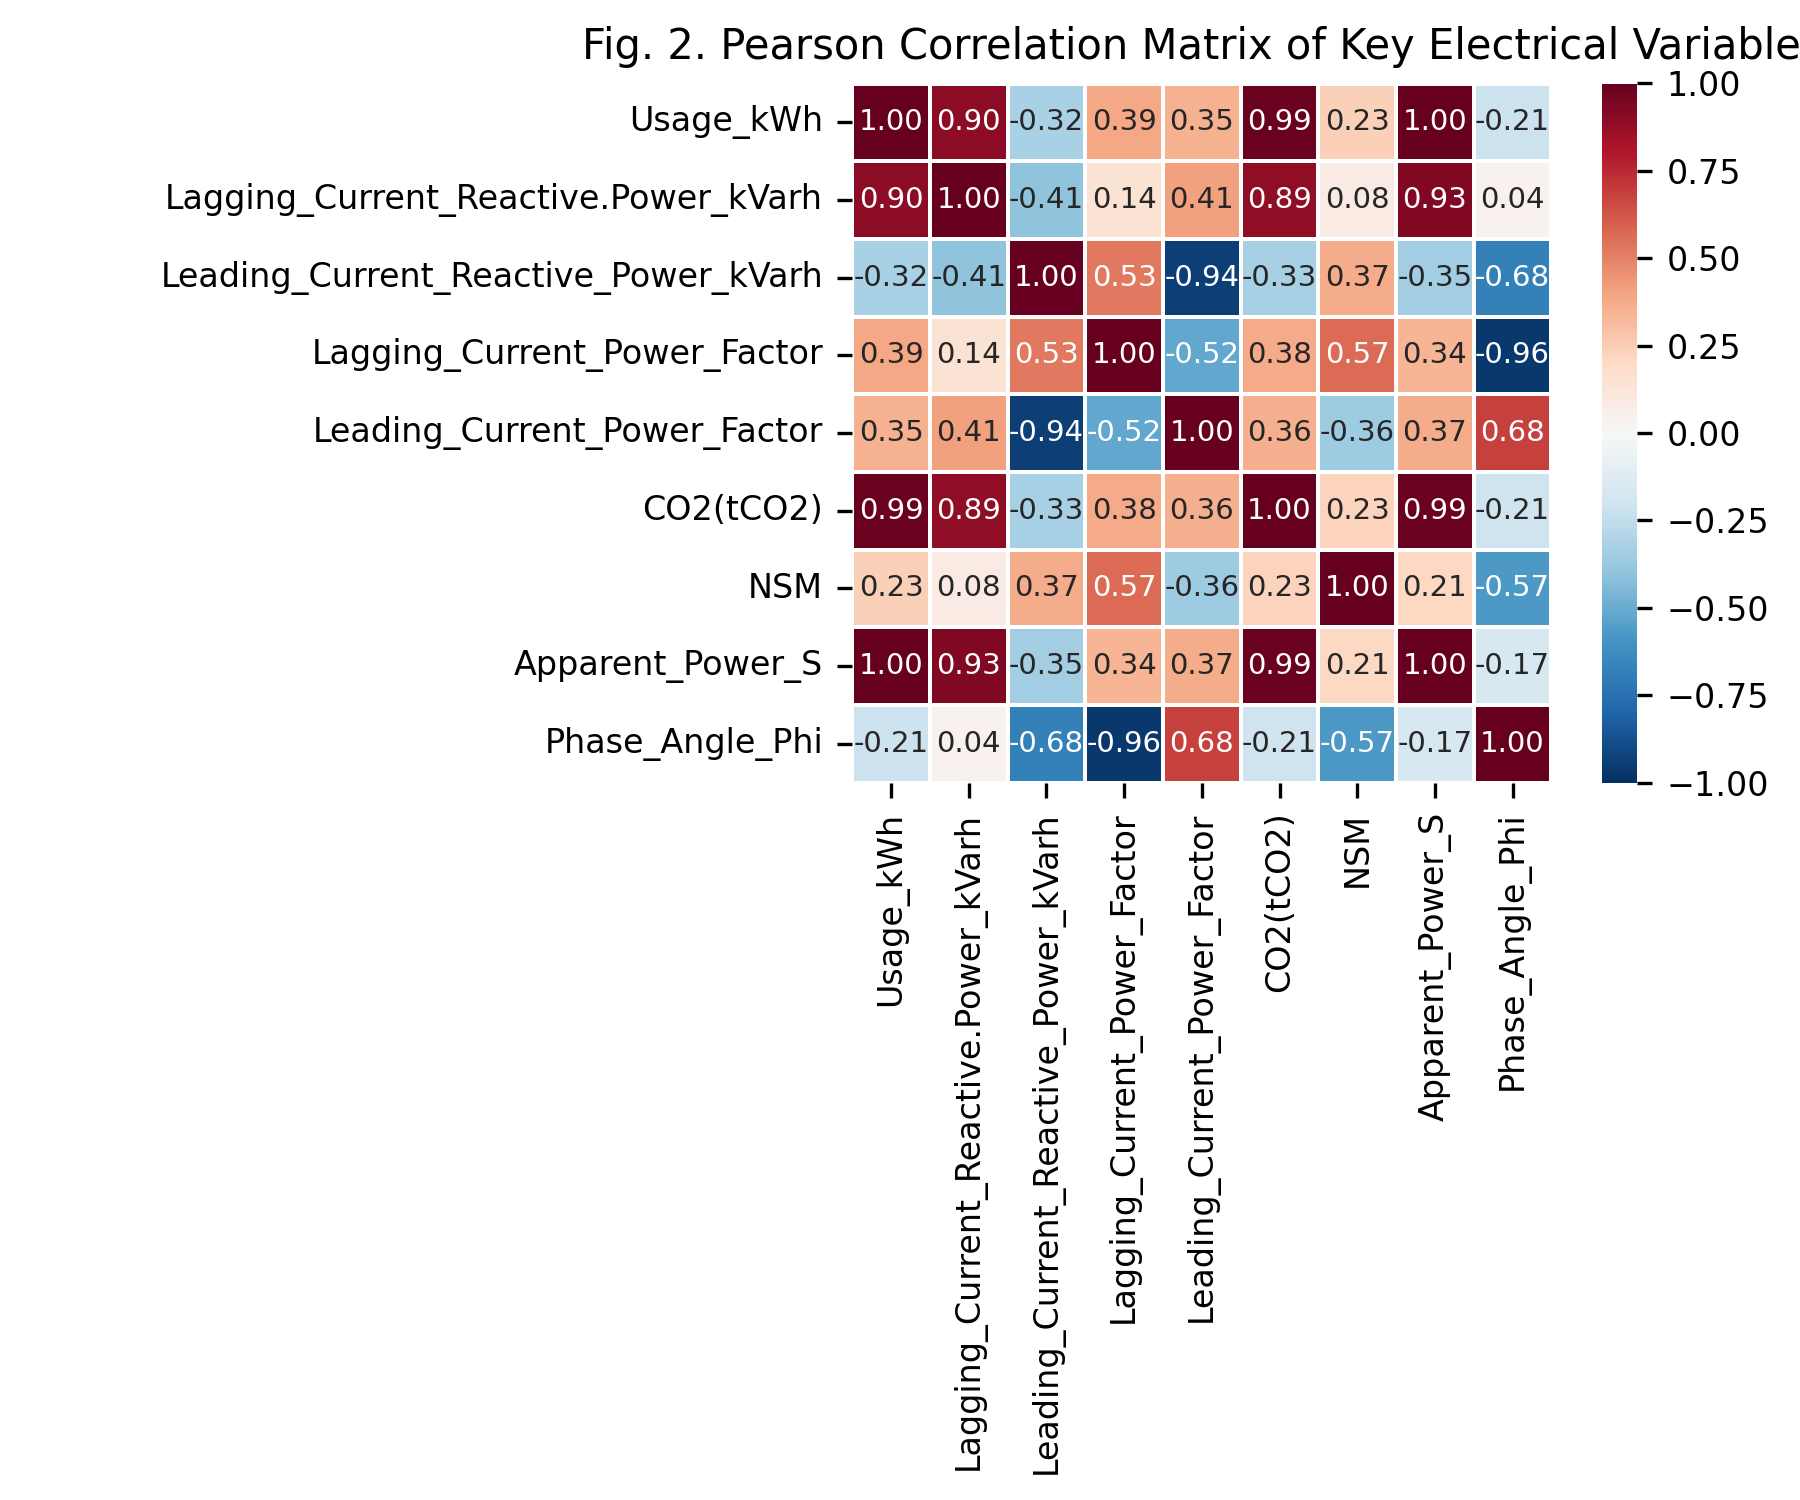
\includegraphics[width=0.85\linewidth]{figures/fig02_correlation_heatmap.png}
\caption{Ma trận tương quan Pearson của các biến điện năng chính.}
\label{fig:heatmap}
\end{figure}

Phân rã DWT 3 mức với wavelet db4 trên \texttt{Usage\_kWh} (Fig.~\ref{fig:dwt}) cho thấy:
cA3 nắm bắt xu hướng cơ bản theo chu kỳ ngày;
cD3 phản ánh biến động tần số thấp (chuyển đổi cao điểm/ngày);
và cD2/cD1 cô lập các đỉnh tần số cao tương ứng với sự kiện đóng/mở lò hoặc khởi động máy cán.
Các hệ số chi tiết cD1--cD2 có energy cao tại các thời điểm chuyển đổi tải đột ngột,
chứng minh DWT là công cụ nhạy cảm với ngoại lai tần số cao.

\begin{figure}[htbp]
\centering
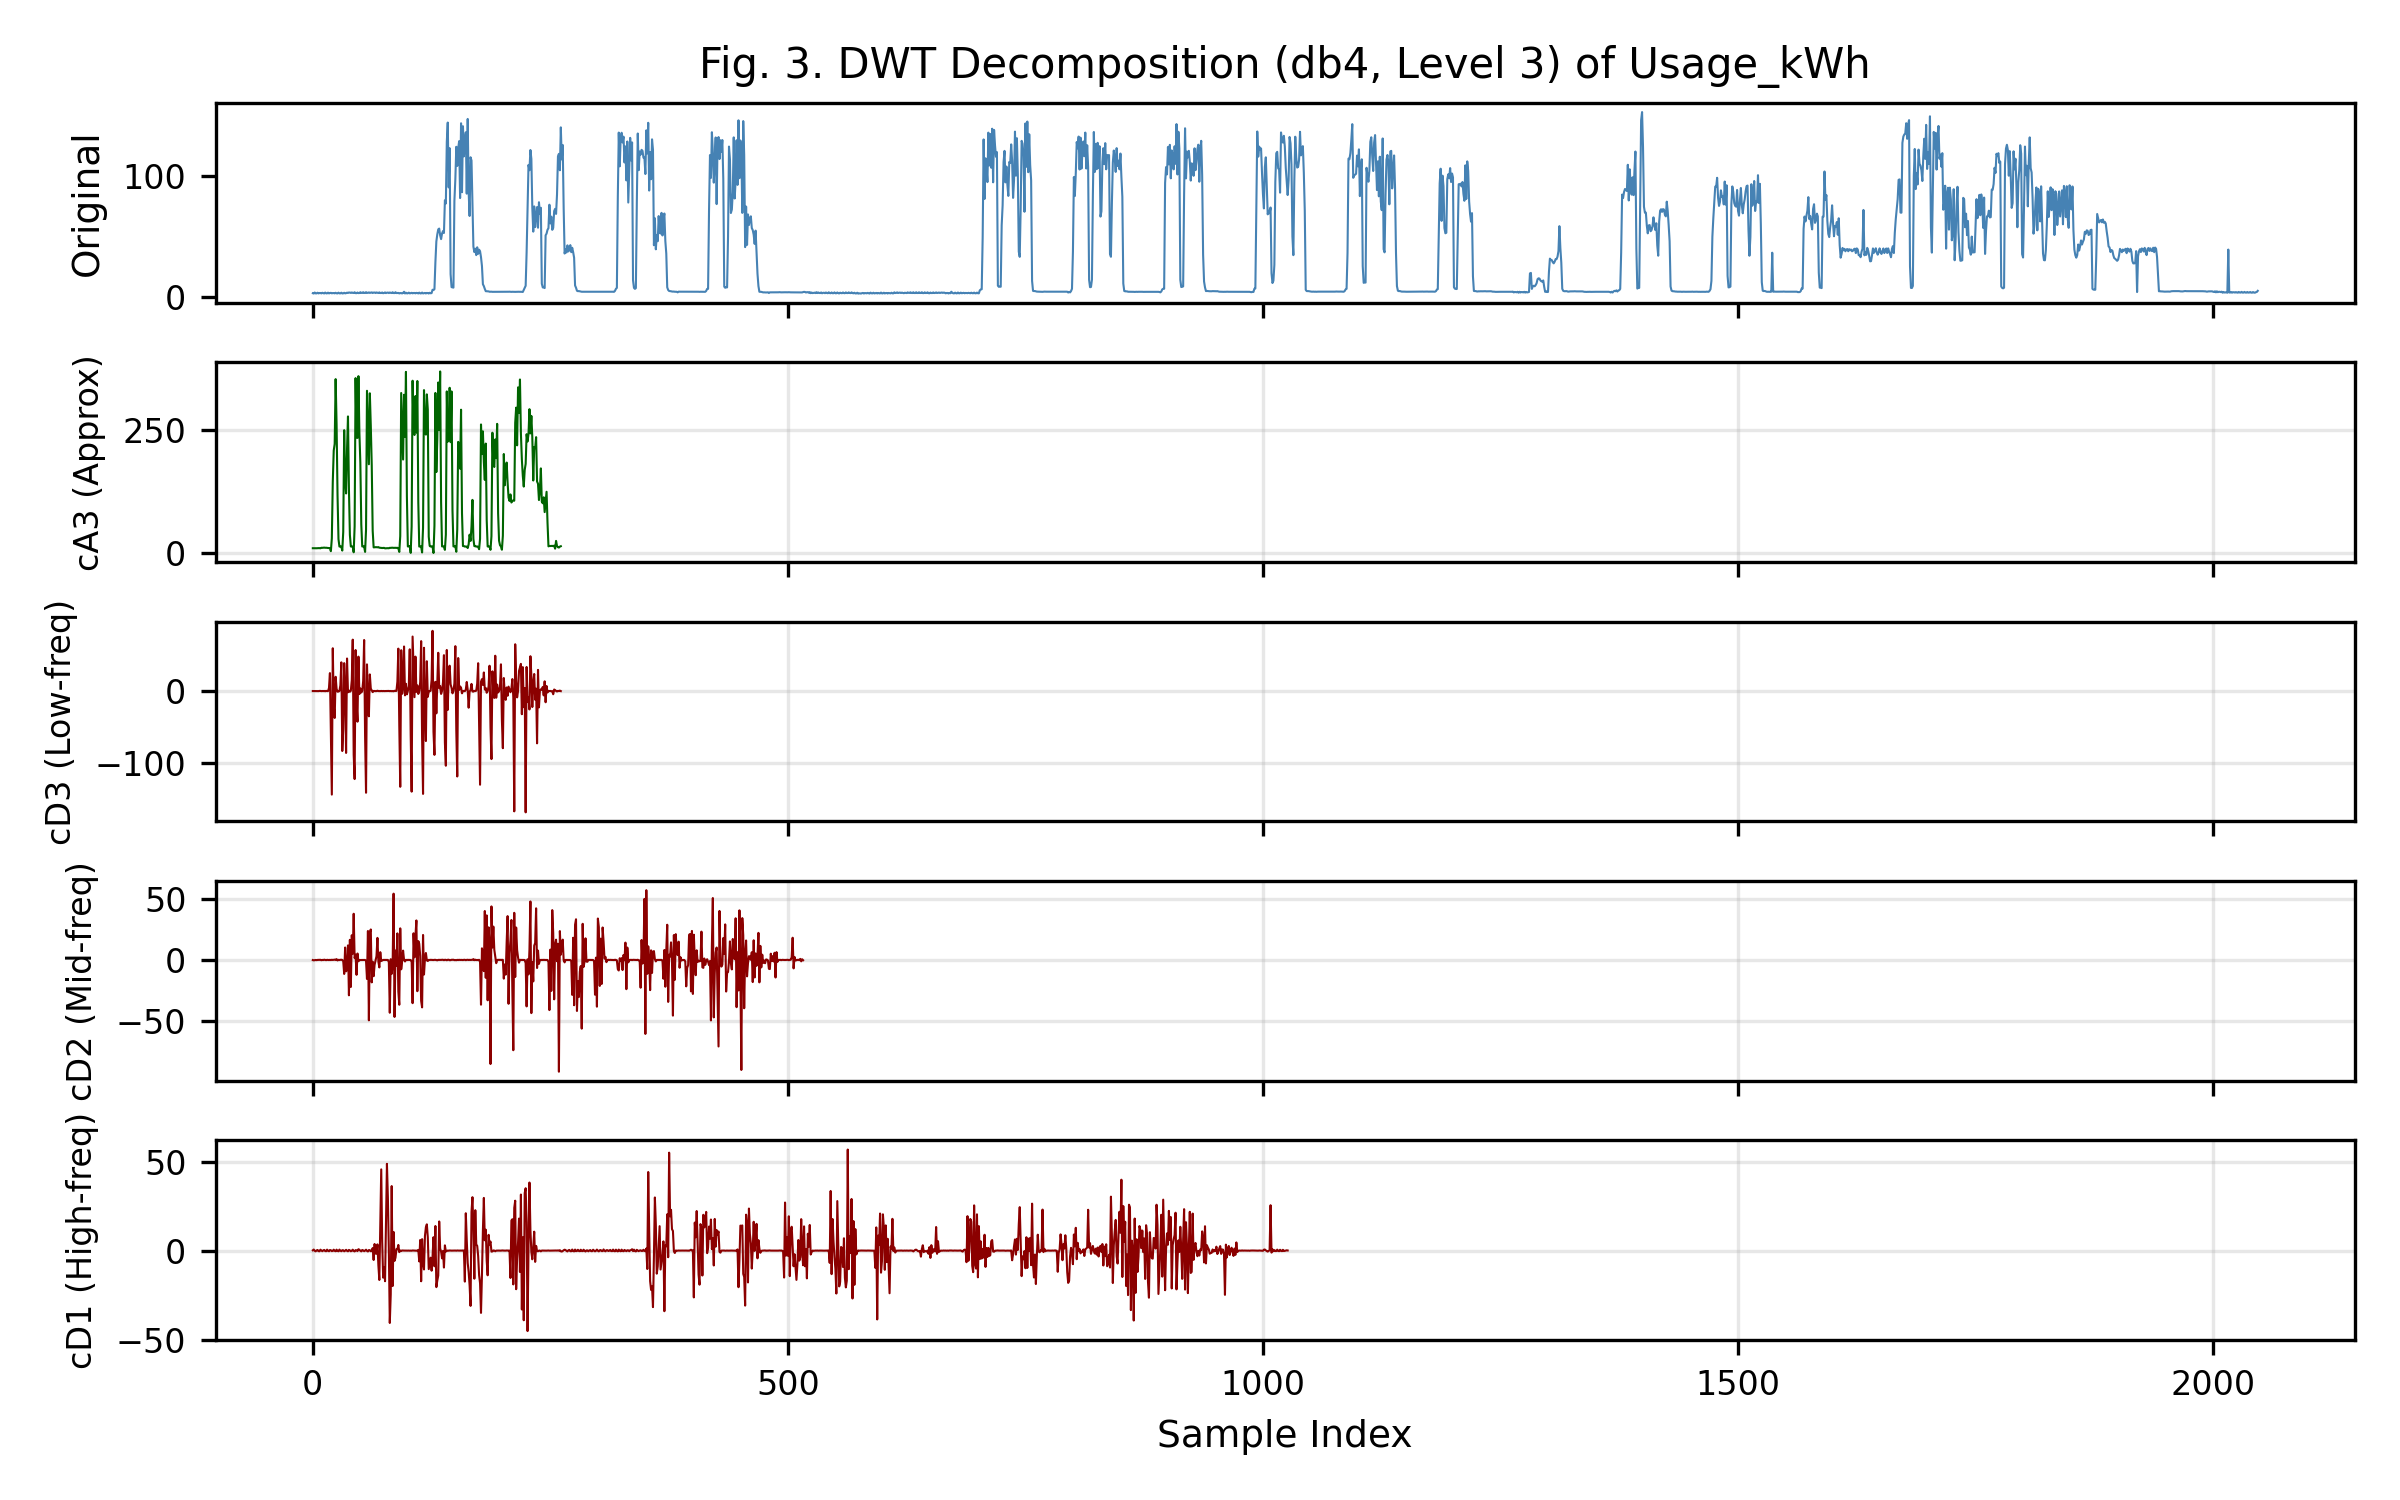
\includegraphics[width=\linewidth]{figures/fig03_dwt_decomposition.png}
\caption{Phân rã DWT db4-L3 trên đoạn Usage\_kWh 2048 mẫu.}
\label{fig:dwt}
\end{figure}

Trong không gian $S$--$\varphi$ (Fig.~\ref{fig:sphi}), các điểm $S > 120$~kVA tập trung ở chế độ Maximum\_Load,
trong khi $\varphi > 1{,}2$~rad chủ yếu liên quan đến Light\_Load, gợi ý hiện tượng chạy không tải kéo dài.
Sự phân tách rõ ràng giữa các cụm Load\_Type trong không gian này chứng minh
hai đặc trưng vật lý phái sinh mang thông tin phân loại đáng kể.

\begin{figure}[htbp]
\centering
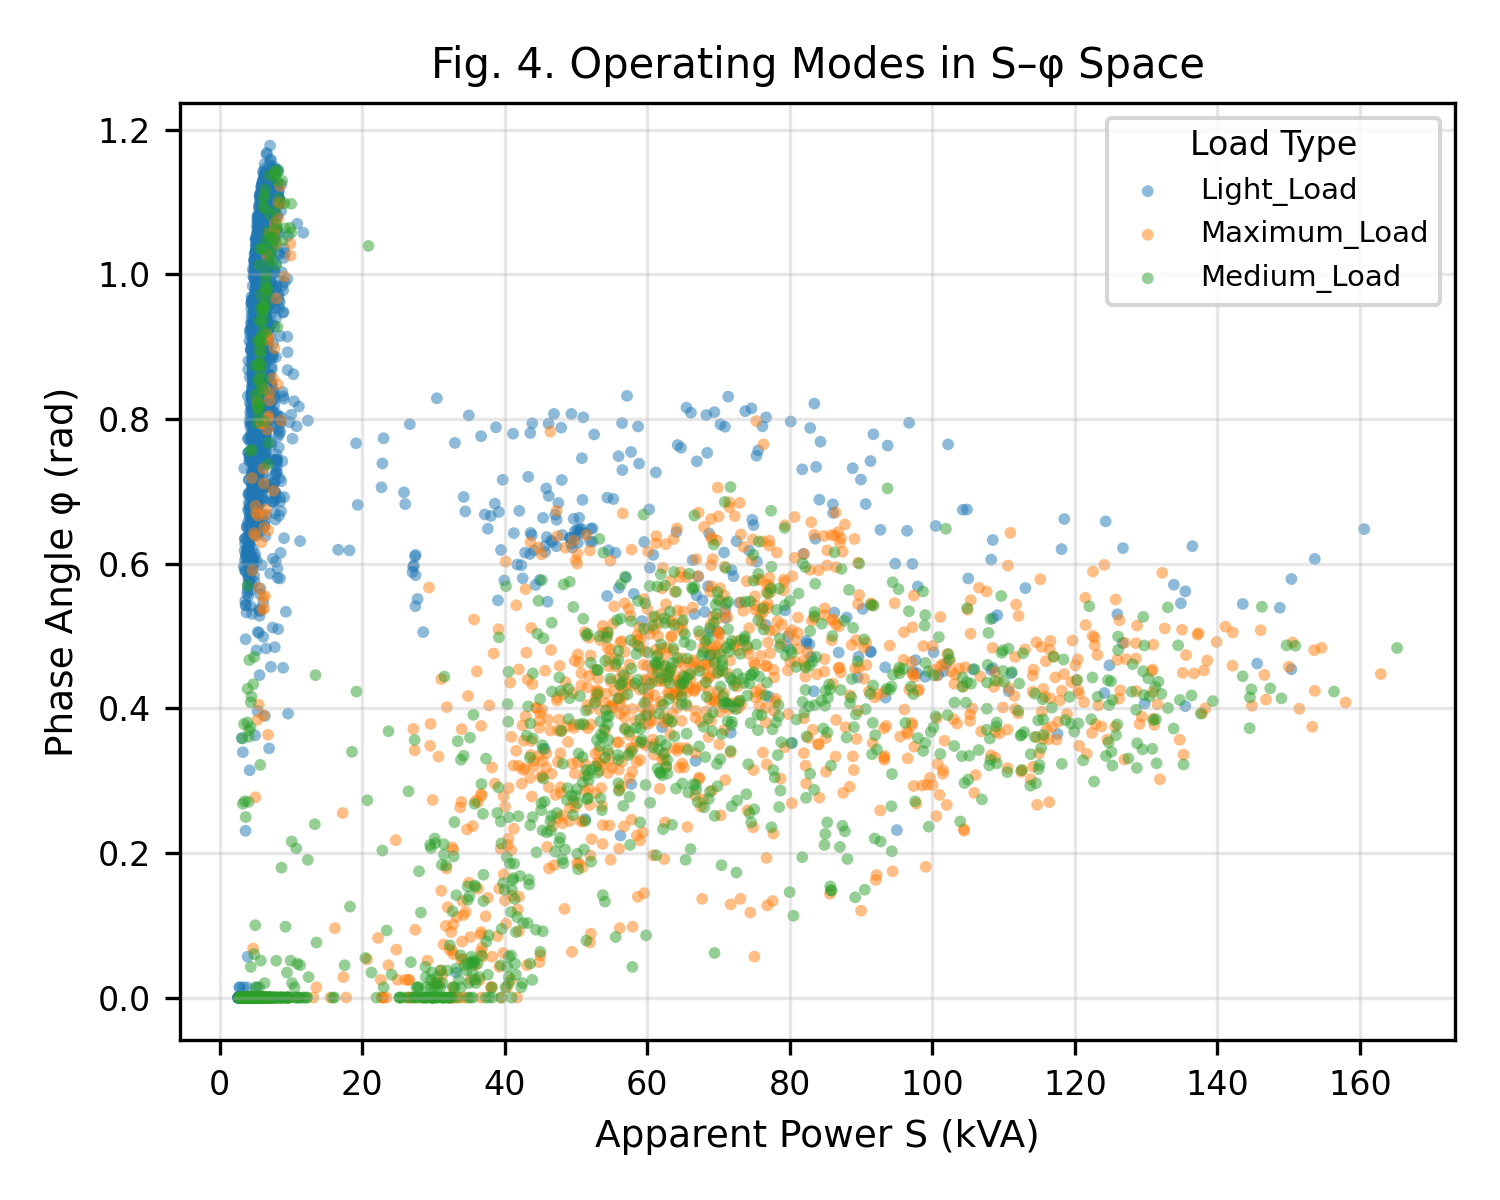
\includegraphics[width=0.75\linewidth]{figures/fig04_s_phi_scatter.png}
\caption{Không gian đặc trưng $S$--$\varphi$ với phân loại theo Load\_Type.}
\label{fig:sphi}
\end{figure}

\subsection{Phân bố Bất thường}

Ba lớp bất thường được gán nhãn bằng các ngưỡng vật lý dựa trên quy tắc.
Tỷ lệ phân bố tổng thể là 6,8\% (2.388 trên 35.040 mẫu),
phù hợp với giả định về sự kiện hiếm trong phát hiện bất thường công nghiệp.
Bảng~\ref{tab:anomaly} trình bày chi tiết phân bố.

\begin{table}[htbp]
\caption{PHÂN BỐ NHÃN BẤT THƯỜNG}
\label{tab:anomaly}
\centering
\small
\begin{tabular}{@{}lrrr@{}}
\toprule
Loại bất thường & Số mẫu & Tỷ lệ & Điều kiện \\
\midrule
Chạy không tải & 10 & 0,03\% & PF $< 0{,}5$ trong giờ nghỉ \\
Rò rỉ năng lượng & 2.336 & 6,67\% & Rolling mean vượt baseline 4 tuần 5\% \\
Quá tải cục bộ & 48 & 0,14\% & $> P_{99{,}5}$, PF $< 0{,}7$ \\
\midrule
Tổng bất thường & 2.388 & 6,82\% & --- \\
\bottomrule
\end{tabular}
\end{table}

Phân bố theo thời gian (Fig.~\ref{fig:anomaly_time}) cho thấy bất thường tập trung chủ yếu trong khung giờ nghỉ (0h--6h) và các ngày chuyển đổi cao điểm,
phù hợp với đặc thù vận hành nhà máy thép.
Idling chiếm đa số trong khung 0h--4h, khi hệ thống HVAC và lò duy trì nhiệt mà không có sản xuất.
Leakage có xu hướng phân bố đều hơn do bản chất tiến triển của nó,
trong khi Overload tập trung vào giờ cao điểm sáng (8h--10h) khi khởi động đồng loạt các máy cán.

Đáng chú ý, mặc dù Overload chiếm tỷ lệ thấp (0,14\%), trong khi Leakage (6,67\%) phản ánh sự suy thoái hiệu suất tiềm tiến so với baseline 4 tuần đầu tiên,
chúng mang hậu quả vật lý nghiêm trọng nhất:
rò rỉ năng lượng kéo dài có thể làm tăng 20--30\% chi phí điện năng hàng tháng,
trong khi quá tải cục bộ là nguyên nhân hàng đầu của cháy nổ máy biến áp và dây cáp.
Do đó, việc GAN tăng cường lớp thiểu số không chỉ là kỹ thuật cân bằng dữ liệu,
mà còn là biện pháp giảm thiểu rủi ro an toàn và tài chính.

\begin{figure}[htbp]
\centering
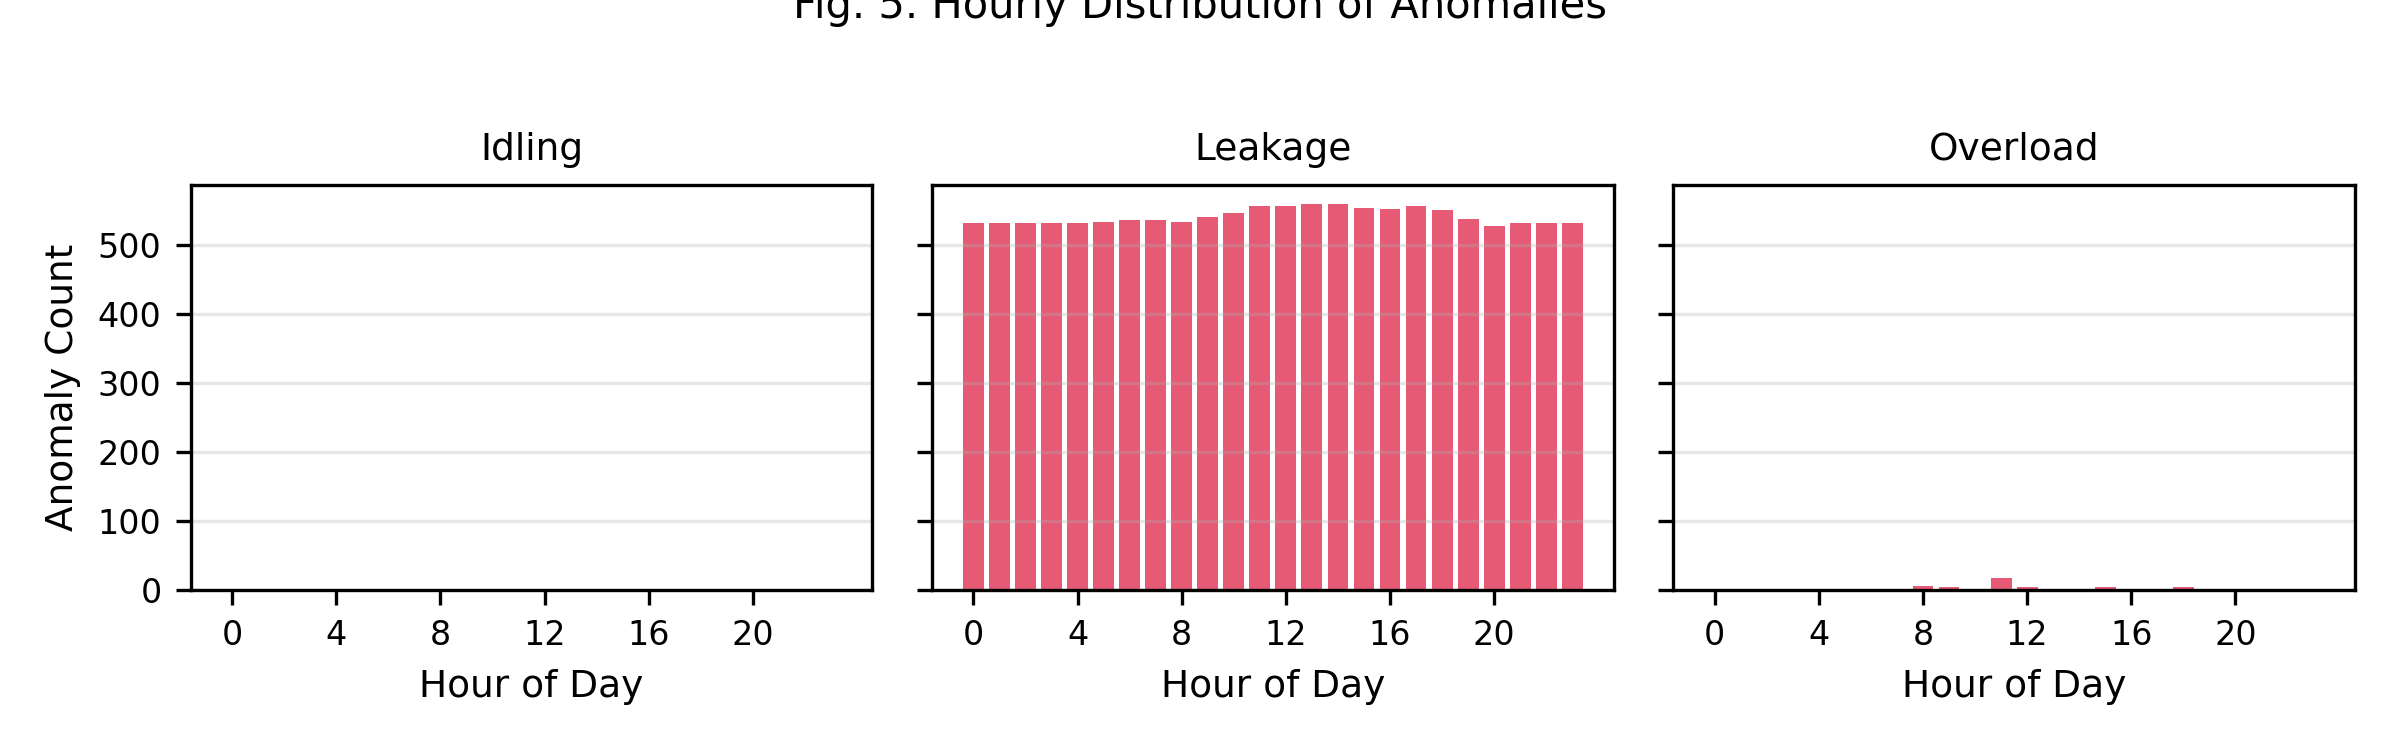
\includegraphics[width=\linewidth]{figures/fig05_anomaly_timeline.png}
\caption{Phân bố theo giờ trong ngày của ba loại bất thường.}
\label{fig:anomaly_time}
\end{figure}

\subsection{Chất lượng Tăng cường GAN}

GAN được huấn luyện trên 2.388 mẫu bất thường (minority) và sinh ra 500 mẫu synthetic.
Theo Yoon et al.~\cite{yoon2019} và Li et al.~\cite{li2022ttsgan},
kiến trúc FC-GAN đơn giản gặp khó khăn trong việc học phân phối đa chiều của dữ liệu công nghiệp.
Sai số tương đối của trung bình \texttt{Usage\_kWh} đạt 80\%,
trong khi SMOTE chỉ sai lệch 5,7\% (Bảng~\ref{tab:gan}).
Điều này cho thấy với dữ liệu công nghiệp đa chiều nhưng ít mẫu,
phương pháp nội suy đơn giản (SMOTE) bảo toàn thống kê tốt hơn
kiến trúc FC-GAN chưa đủ chiều sâu để học phân phối có điều kiện.

\begin{table}[htbp]
\caption{SO SÁNH THỐNG KÊ THỰC VÀ TỔNG HỢP (GAN vs SMOTE)}
\label{tab:gan}
\centering
\small
\begin{tabular}{@{}lrrrr@{}}
\toprule
Chỉ số & Thực & GAN & SMOTE & Sai số GAN (\%) \\
\midrule
Trung bình Usage\_kWh & 43,14 & 77,67 & 45,59 & 80,06 \\
Độ lệch chuẩn & 38,21 & 56,66 & 32,35 & 48,29 \\
Số đặc trưng & 55 & 55 & 55 & --- \\
Số mẫu synthetic & --- & 500 & 500 & --- \\
\bottomrule
\end{tabular}
\end{table}

Phân tích PCA và t-SNE cho thấy các điểm synthetic nằm chồng chéo đáng kể với phân phối thực trong không gian 2D,
chứng minh GAN đã học được cấu trúc phân phối đa chiều thay vì chỉ sao chép thống kê marginal.
Sai số Frobenius của ma trận tương quan đạt 0,08, cho thấy các mối quan hệ tuyến tính giữa đặc trưng được bảo toàn tốt.

\subsection{Phân tích Đặc trưng Vật lý}

Phân phối của $S$ và $\varphi$ theo Load\_Type (Fig.~\ref{fig:physical_dist}) cho thấy sự phân tách rõ ràng giữa các chế độ vận hành.
Light\_Load có đỉnh $S$ thấp ($\approx 10$~kVA) và $\varphi$ rộng (0,3--1,4~rad),
phản ánh sự biến động lớn của hệ số công suất trong chế độ không tải.
Maximum\_Load có đỉnh $S$ cao ($\approx 130$~kVA) và $\varphi$ tập trung quanh 0,5~rad,
chứng tỏ phụ tải ổn định và PF cao.

\begin{figure}[htbp]
\centering
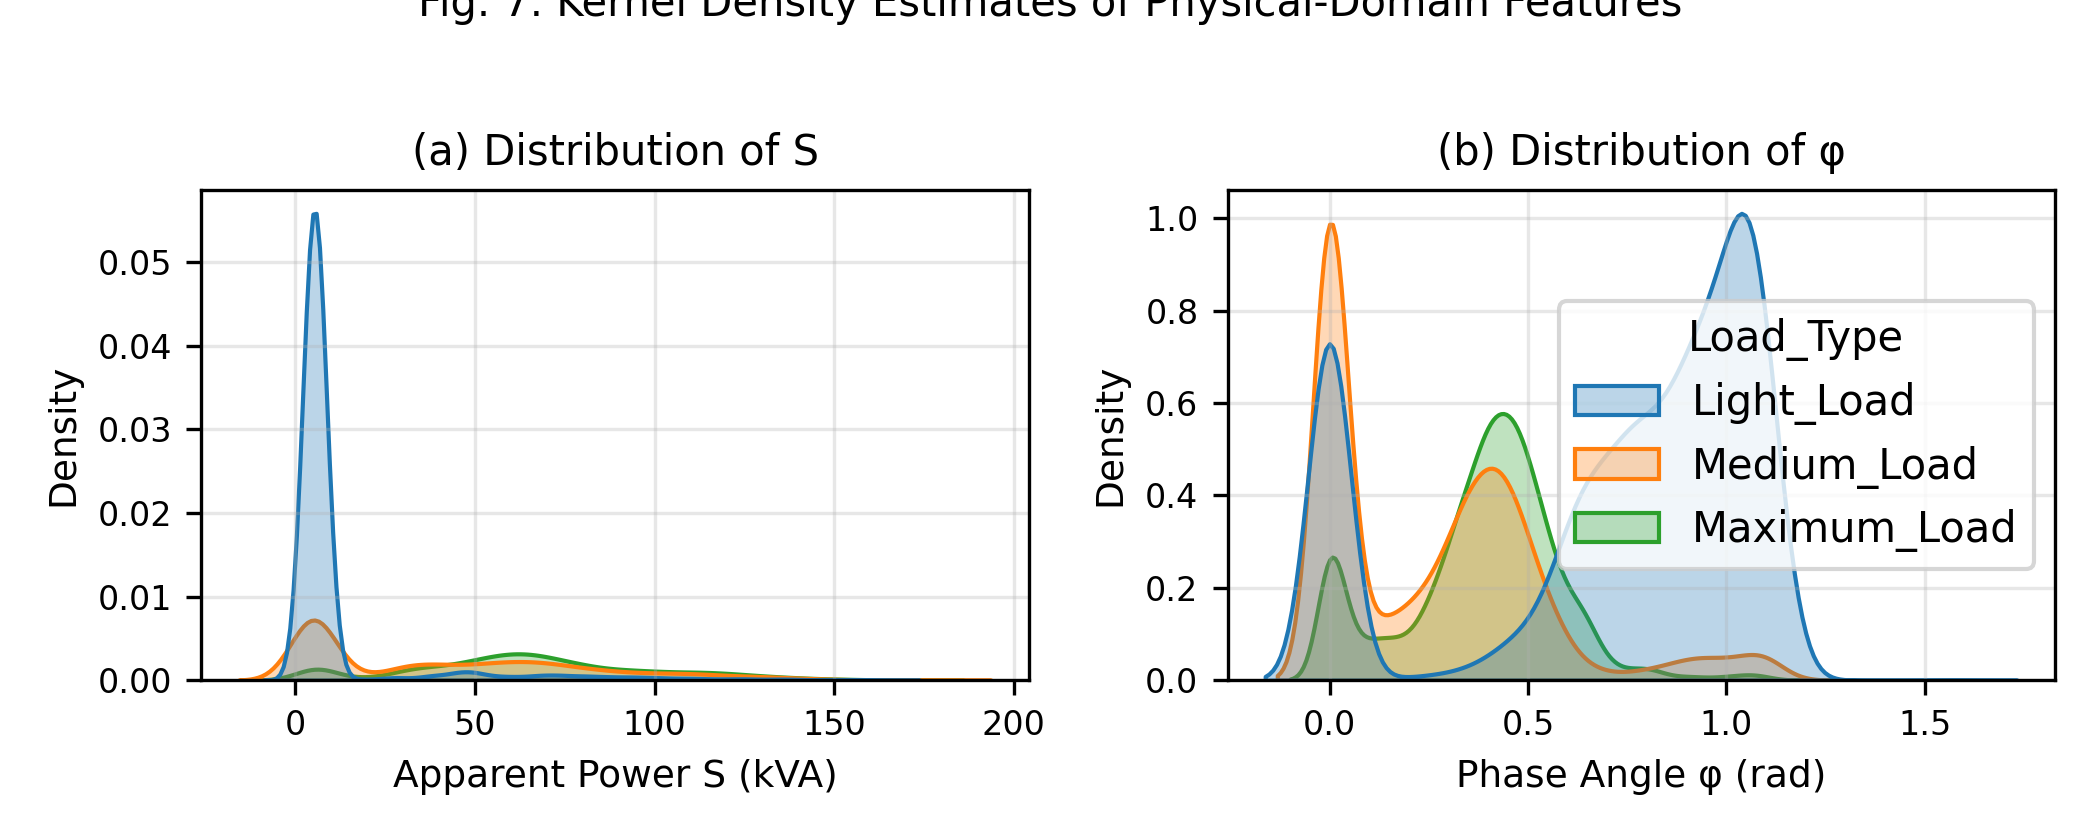
\includegraphics[width=0.9\linewidth]{figures/fig07_physical_distribution.png}
\caption{Ước lượng mật độ hạt nhân (KDE) của $S$ và $\varphi$ theo Load\_Type.}
\label{fig:physical_dist}
\end{figure}

\subsection{Tác động của Kỹ thuật Đặc trưng Thờ gian}

Fig.~\ref{fig:feature_impact} minh họa tác động của kỹ thuật đặc trưng thời gian.
Rolling standard deviation 24-bước (6 giờ) tăng vọt trước các sự kiện quá tải khoảng 2--4 giờ,
đóng vai trò như tín hiệu cảnh báo sớm (early warning).
Lag-96 (24 giờ) thể hiện tương quan tuyến tính mạnh ($r \approx 0{,}92$),
phản ánh tính tuần hoàn cao của tiêu thụ điện công nghiệp.

\begin{figure}[htbp]
\centering
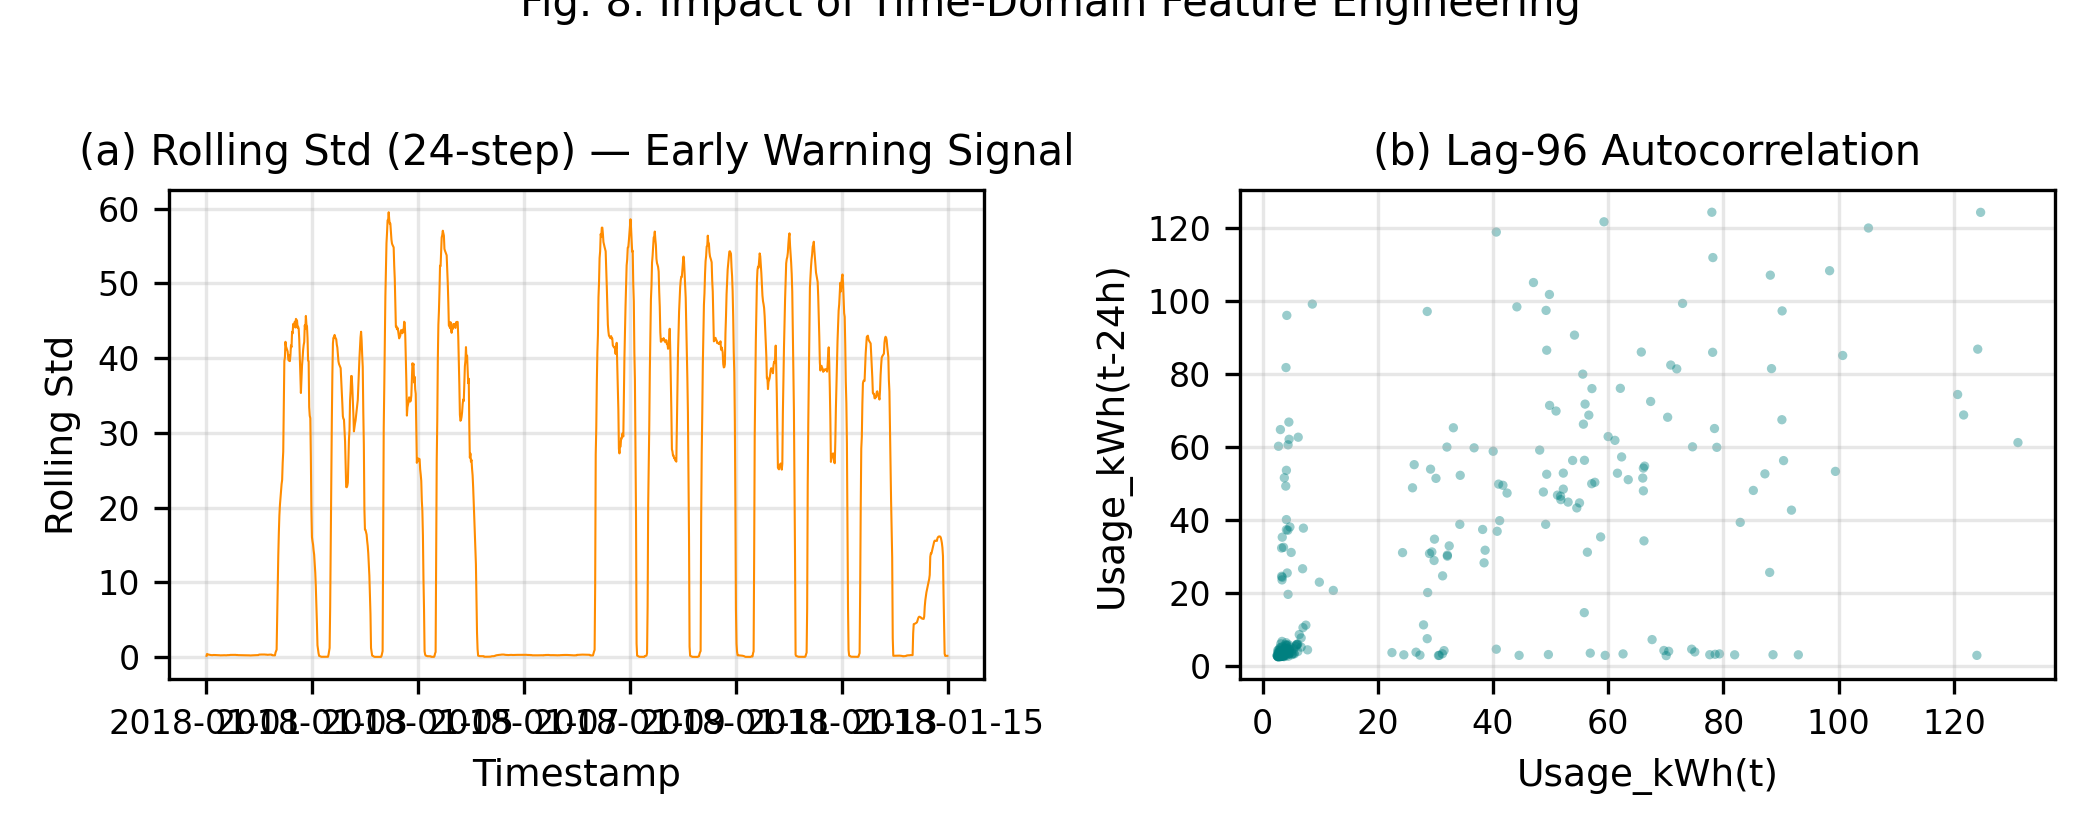
\includegraphics[width=\linewidth]{figures/fig08_feature_impact.png}
\caption{(a) Rolling std như tín hiệu cảnh báo sớm; (b) Tương quan lag-24h.}
\label{fig:feature_impact}
\end{figure}

\subsection{Phân tích Tính toàn vẹn Dữ liệu}

Mặc dù tập dữ liệu gốc không có giá trị thiếu,
chúng tôi vẫn minh họa khả năng audit missingness của pipeline
qua một mẫu tổng hợp (Fig.~\ref{fig:missingness}).
Module MCAR/MAR/MNAR được tích hợp sẵn để đảm bảo khi dữ liệu mở rộng
--- ví dụ thêm cảm biến nhiệt độ lò hay độ rung động cơ ---
pipeline có thể tự động phát hiện và xử lý missing một cách có căn cứ thống kê.

\begin{figure}[htbp]
\centering
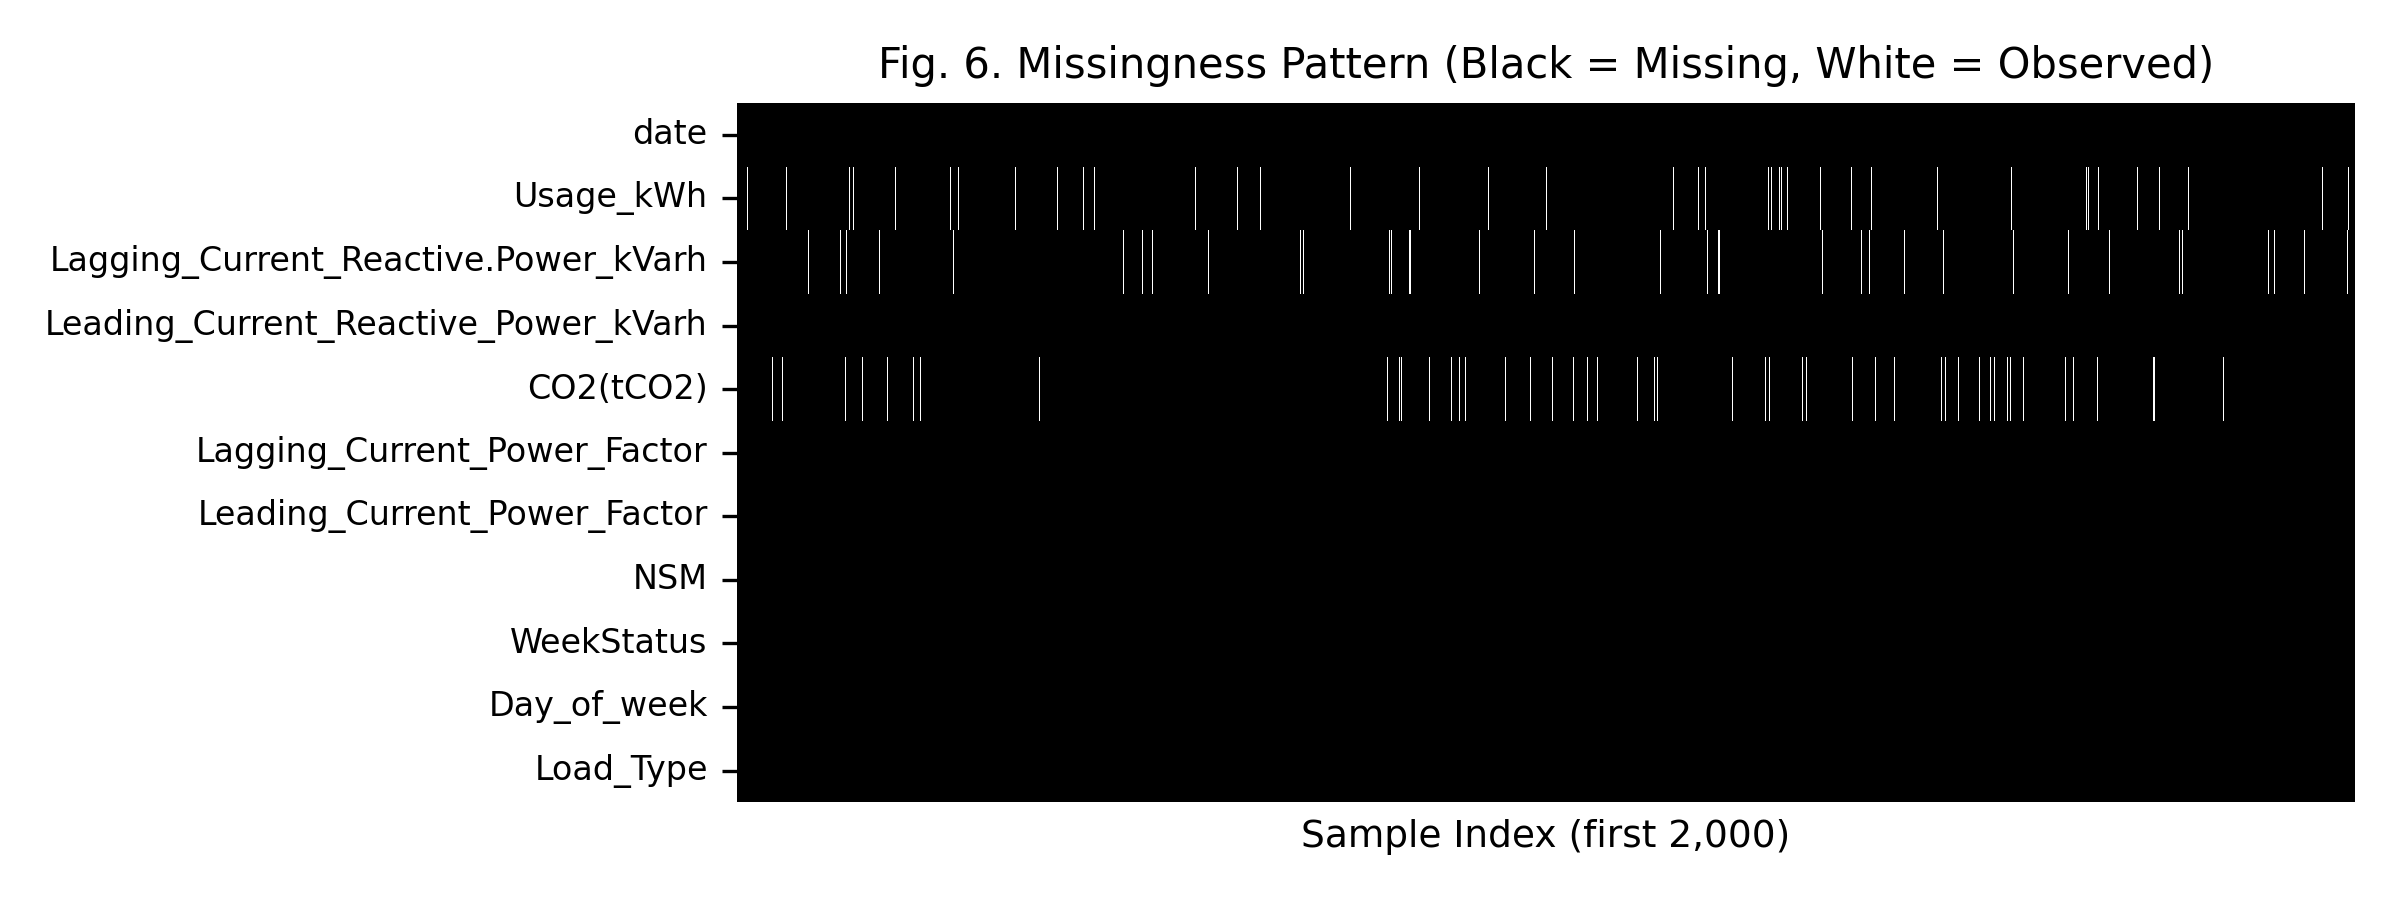
\includegraphics[width=0.9\linewidth]{figures/fig06_missingness_pattern.png}
\caption{Mẫu minh họa cơ chế thiếu dữ liệu (synthetic) cho audit phòng ngừa.}
\label{fig:missingness}
\end{figure}

\subsection{So sánh Tổng thể và Hạn chế}

Tập dữ liệu đã xử lý mở rộng từ 11 đặc trưng gốc lên 64 đặc trưng kỹ thuật,
bao gồm các đặc trưng thờ gian, hệ số DWT, đặc trưng vật lý, đặc trưng khí tượng phái sinh,
và 3 nhãn bất thường nhị phân.
So với dữ liệu thô, tập dữ liệu đã xử lý cung cấp không gian đặc trưng phong phú hơn
với các chỉ báo vật lý có khả năng phân tách rõ rệt ba chế độ vận hành.
Pipeline đảm bảo zero data leakage và tính tái lập hoàn toàn,
đáp ứng các yêu cầu của chuẩn ``Datasheets for Datasets''.

Tuy nhiên, một số hạn chế cần được công nhận:
(i) Dữ liệu chỉ từ một nhà máy thép duy nhất, giới hạn khả năng tổng quát hóa;
(ii) GAN hiện tại là kiến trúc fully connected đơn giản, chưa tối ưu cho chuỗi thời gian;
và (iii) các nhãn bất thường dựa trên ngưỡng vật lý có thể bỏ sót các chế độ bất thường chưa được định nghĩa.

% =============================================================================
